%\showthe\columnwidth
\chapter{Preâmbulo Teórico}

Para que possamos fazer uma análise comparativa entre duas estratégias estatísticas, temos que, antes, entender suas diferenças e similaridades, bem como as características dos dados com os quais estamos lidando.

Assim, este capítulo será dividido em duas grandes seções, uma destinada à apresentação das bases de imagens utilizadas, outra destinada à discussão sobre as qualidades dos dados nessas bases.

\section{As bases de dados}\label{sec:imdb}

Para o cumprimento desse trabalho, escolhemos duas bases de imagens diferentes, que chamaremos simplesmente Toyama e LIVE.

A base Toyama é, na verdade, chamada \textbf{IRCCyN/IVC-Toyama database (LCD)} e tem acesso franqueado no site ~\cite{Tourancheau2008} do IRCCyN (\emph{Institut de Recherche en Communications et Cybernétique de Nantes}), da Universidade de Nantes, na França.

A base LIVE é oficialmente conhecida como \textbf{LIVE Image Quality Assessment Database} e tem acesso também franqueado no site \cite{livedb} do LIVE (\emph{Laboratory for Image \& Video Engineering}). Utilizamos sua \emph{release 1} nesse trabalho, por ser a única que disponibilizava dados de avaliação subjetiva para compressão JPEG.

Ambas as bases possuem imagens originais (não degradadas) e um determinado número de imagens degradadas com diferentes tipos e graus de degradação; nosso trabalho se concentra na degradação do tipo JPEG, em todos os graus disponíveis nas bases. A \autoref{tab:bds} apresenta as principais características de ambas as bases. 

\begin{table}[htb]
	\footnotesize
	\caption[Características das Imagens das Bases de Dados]{Características das Imagens das Bases de Dados}
	\label{tab:bds}
	\centering
 	\begin{tabular}{ l | c | c } %\toprule[1.5pt]
% \begin{minipage}{\linewidth}
% 	\captionof{table}{Características das Imagens nas Bases de Dados} \label{tab:bds}
% 	\begin{tabular}{ l | c | c } %\toprule[1.5pt]
							&	\textbf{Toyama}			&	\textbf{LIVE} 		\\\hline % \midrule
		Número Total de Imagens	$T_i$		&	$98$				&	$204$	  		\\ % \midrule
		Número de Imagens de Referência $I_r$	& 	$14$				&	$29$		  	\\
		Número de Imagens degradadas $I_d$	&	$84$				&	$175$	  		\\
		Resolução das Imagens na base		& 	$768 \times 512$ pixels 	&	$768 \times 512$ pixels	\\
		Profundidade de cor			&	$24bits/pixel$			&	$24bits/pixel$ 		\\
		Formato das imagens cedidas		&	BMP				&	BMP		  	\\
		Tipo de degradação			&	JPEG				&	JPEG		  	\\
		Graus de degradação aplicados		& $15$, $20$, $27$, $37$, $55$, $79$ 	& 	não informado 		\\
		Diversidade de graus de degradação	&	$6$ taxas			&  	não informado 		\\
		Faixa de valores de avaliação		& 	$[1, 5]$			& 	$[0, 100]$		\\
		Categorias de Qualidade			&	$5$				& 	$5$			\\
		Sessões de Avaliação distintas		&	$1$				& 	$2$			\\
		
%		\bottomrule[1.25pt]
	\end {tabular}\par
	\legend{Fontes: \cite{livedb,Tourancheau2008}}
\end{table}

As \autoref{fig:liveref} e \autoref{fig:livedist} apresentam exemplos de figuras disponíveis na base LIVE; já as figuras \autoref{fig:toyaref} e \autoref{fig:toyadist} provém da base Toyama. As imagens à esquerda são imagens de referência, não-corrompidas, enquanto as da direita já passaram por compressão JPEG.

\begin{figure}[htb]
 \label{fig:liveex}
 \centering
  \begin{minipage}{0.48\textwidth}
    \centering
    \caption{Imagem de referência LIVE} \label{fig:liveref}
    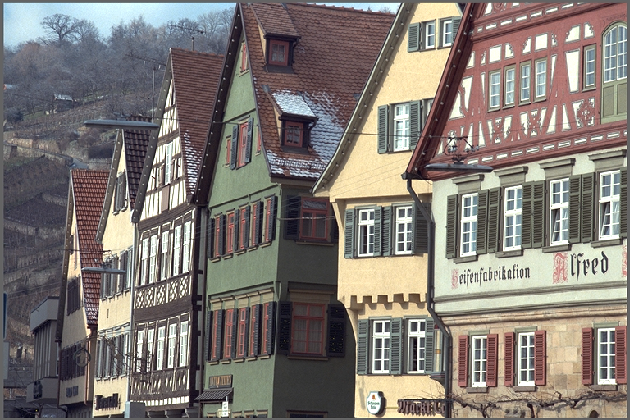
\includegraphics[width=\textwidth]{../img/liveref66.pdf}
    \legend{Fonte: \cite{livedb}}
  \end{minipage}
  \hfill
  \begin{minipage}{0.48\textwidth}
    \centering
    \caption{Imagem distorcida LIVE} \label{fig:livedist}
    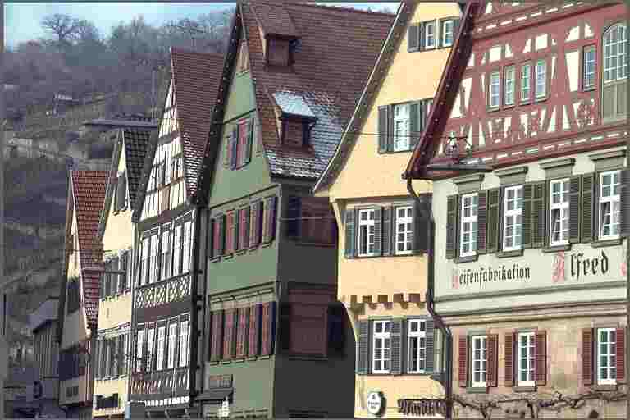
\includegraphics[width=\textwidth]{../img/liveref90.pdf}
    \legend{Fonte: \cite{livedb}}
  \end{minipage}
\end{figure}

Segundo a LIVE, o estudo que gerou as bases conduziu duas sessões de avaliação distintas. Os pesquisadores tiveram o cuidado de apresentar, em ambas as sessões, todas as imagens de referência e suas respectivas distorções. A quantidade de sujeitos no experimento foi diferente em cada sessão: na primeira, houve vinte sujeitos, apenas treze na segunda. Os pesquisadores afirmam que a escolha das imagens para o estudo foi tal que possibilitaria uma distribuição aproximadamente uniforme das notas de avaliação, o que pode ser visualizado no histograma da \autoref{graf:liveHist}, gerado diretamente a partir dos valores das notas. Não foi imposta restrição de distância de visualização para a avaliação e as imagens foram mostradas aos sujeitos aleatoriamente. Para emitir suas opiniões, os sujeitos poderiam levar o tempo que necessitassem, mas poderiam visualizar cada imagem apenas uma vez. Os pesquisadores promoveram uma pequena sessão de treinamento antes do início de cada sessão de avaliação. Estas informações e maiores detalhes podem ser obtidos no \emph{site} da referida base.\cite{livedb}

\begin{figure}[htb]
%	\label{graf:liveHist}
	\centering
	\begin{minipage}{.8\textwidth}
		\caption{Histograma de avaliação subjetiva  --- LIVE}\label{graf:liveHist}
		\centerline{\includegraphics{../../graphs/L_Hist_OSs.pdf}}
	\legend{Histograma gerado a partir das opiniões dos sujeitos sobre a totalidade das imagens da base}
	\end{minipage}
\end{figure}

\begin{figure}[htb]
 \label{fig:toyaex}
 \centering
  \begin{minipage}{0.48\textwidth}
    \centering
    \caption{Imagem de referência Toyama} \label{fig:toyaref}
    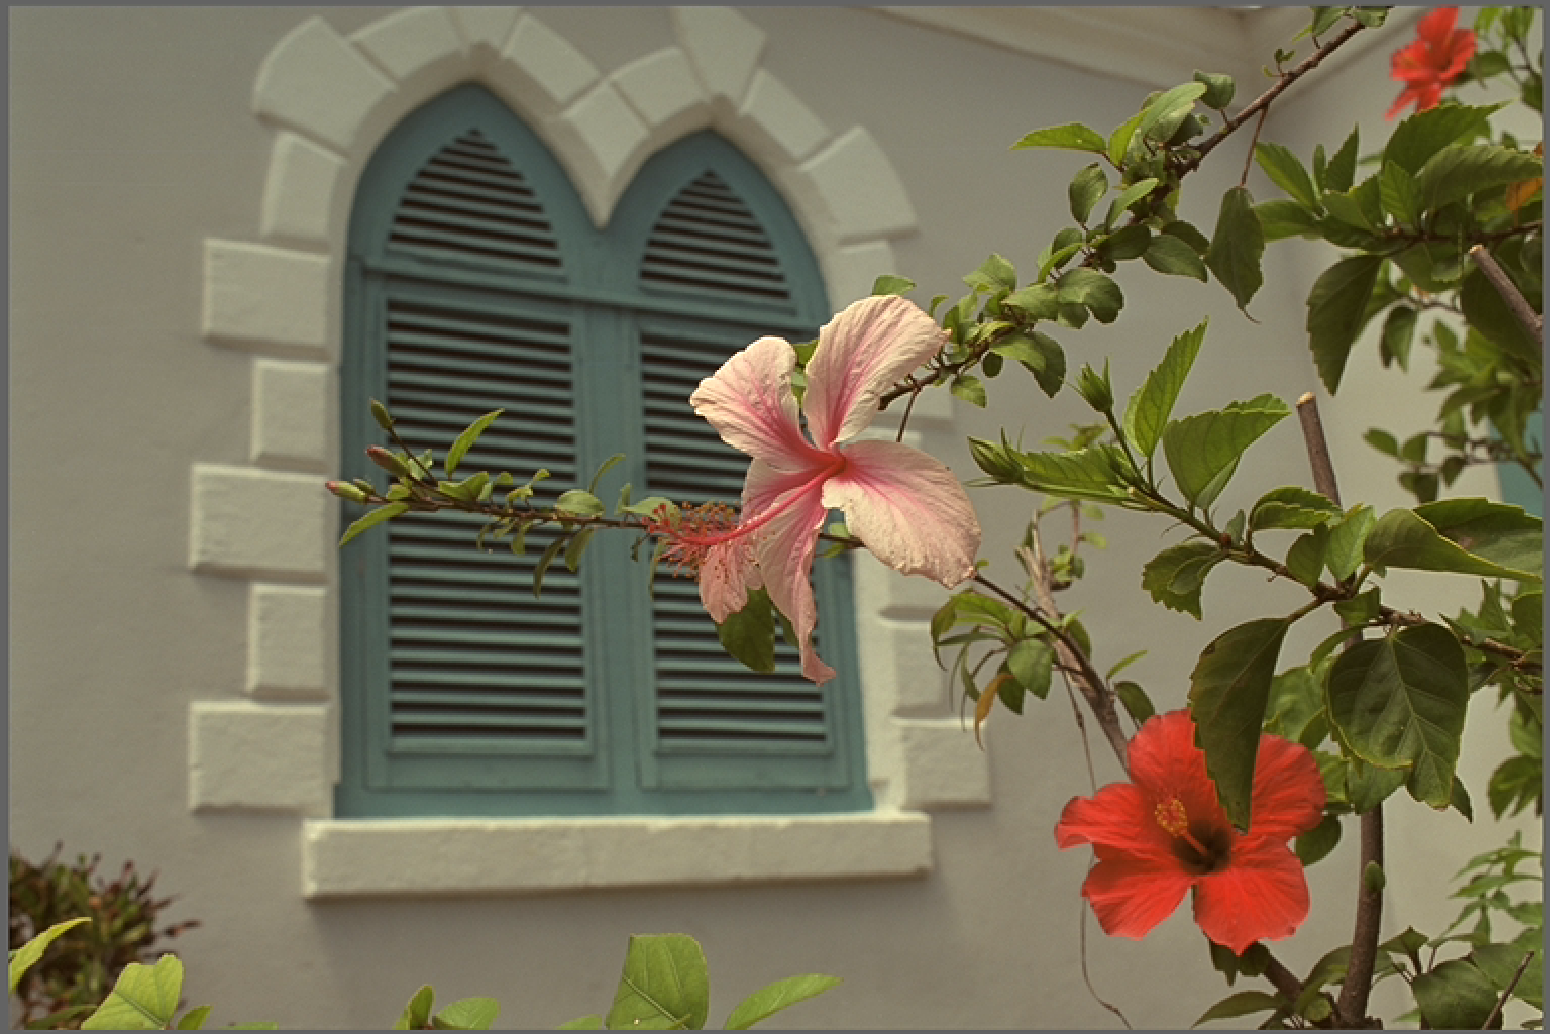
\includegraphics[width=\textwidth]{../img/toyaref07.pdf}
    \legend{Fonte: \cite{Tourancheau2008}}
  \end{minipage}
  \hfill
  \begin{minipage}{0.48\textwidth}
    \centering
    \caption{Imagem distorcida Toyama} \label{fig:toyadist}
    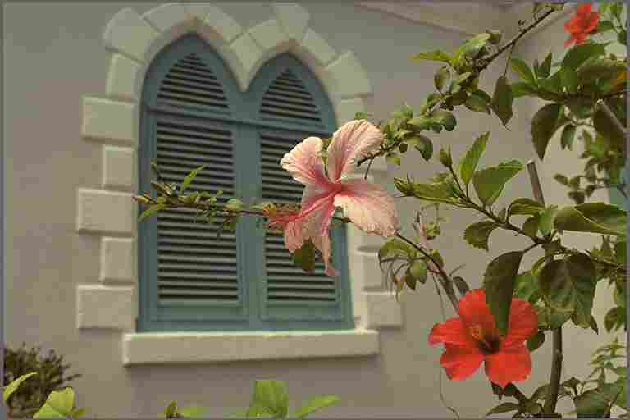
\includegraphics[width=\textwidth]{../img/toyadist07_79.pdf}
    \legend{Fonte: \cite{Tourancheau2008}}
  \end{minipage}
\end{figure}

Segundo o arquivo de informações que acompanha a base Toyama, foram dezesseis não-peritos que avaliaram as imagens dessa base, em sua maioria estudantes, não informando se houve ou não sessões distintas (e por isso assumimos uma única sessão). Da mesma forma que a LIVE, as imagens foram apresentadas aleatoriamente, sem restrição de tempo e também com apenas uma oportunidade de visualização para avaliação de cada imagem. Neste estudo foi imposta a distância de observação igual a quatro vezes a altura da imagem. A Toyama apresenta dezesseis avaliações distintas para cada imagem, totalizando, portanto, dezesseis sujeitos no experimento. O histograma das notas de avaliação das imagens dessa base pode ser observado na \autoref{graf:toyaHist} (também gerado a partir das notas de avaliação).
 

\begin{figure}[htb]
%	\label{graf:liveHist}
	\centering
	\begin{minipage}{.8\textwidth}
		\caption{Histograma de avaliação subjetiva --- Toyama}\label{graf:toyaHist}
		\centerline{\includegraphics{../../graphs/T_Hist_OSs.pdf}}
		\legend{Histograma gerado a partir das opiniões dos sujeitos sobre a totalidade das imagens da base}
	\end{minipage}
\end{figure}

Ambas os grupos de pesquisa deram a seus sujeitos uma escala com as palavras ``\emph{bad}'', ``\emph{poor}'', ``\emph{fair}'', ``\emph{good}'' e ``\emph{excellent}'', mas cada uma associou a essas palavras uma escala diferente. Além de os intervalos de avaliação serem distintos, como pode ser observado na \autoref{tab:bds}, outra diferença se faz digna de nota: a LIVE considera contínuo e linear o domínio de avaliação, enquanto a Toyama considera esse domínio discreto. Ou seja, na LIVE encontraremos notas como $4,55$, ou $9,42$ e na Toyama, apenas os inteiros no intervalo $[1,5]$. A Toyama ainda informa que seus testes foram executados conforme as condições de avaliação apontadas no ITU-R Rec. 500-10 (de março de 2010). Veremos mais detalhes sobre essa recomendação na sessão seguinte.

\section{Avaliação de Qualidade de Imagens}

Como dito no \autoref{chap:intro}, os atuais usos de imagens e vídeos digitais têm sua abrangência amplificada, na medida em que novos serviços surgem no mercado --- e que mais usuários utilizam esses serviços. Isso, como dito, se torna um desafio pra indústria, que precisa encontrar formas cada vez mais econômicas e eficientes de entregar seus produtos (mídias digitais) utilizando a infra-estrutura de comunicação existente e com o mínimo custo computacional e de armazenamento.

Para resolver problemas de armazenamento e tráfego, algoritmos de compressão foram desenvolvidos e são utilizados corriqueiramente. Padrões de compressão, como o JPEG e MPEG (imagem e vídeo, respectivamente), são muito frequentemente utilizados no tráfego de dados via internet. Esses algoritmos podem ser divididos em duas categorias: a dos ``com perdas'' (\emph{lossy}) e a dos ``sem perdas'' (\emph{lossless}).

Exemplos de algoritmos \emph{lossless} para imagens são PNG e TIFF. ``Sem perdas'' significa que, uma vez descompactas, as imagens resultantes guardam as mesmas características das images originais --- o mesmo volume de dados dentro da mesma conformação espacial. Exemplos de algoritmos \emph{lossless}, que consideram a perda de informação como razoável e atingem taxas de compressão mais elevadas, são os já citados JPEG e MPEG.

A nós interessam considerações sobre os métodos de compressão com perdas, já que eles são capazes de economizar mais banda da rede de comunicação e otimizar ainda mais o armazenamento, em relação aos métodos sem perdas. Estabelece-se então uma relação de compromisso entre compactação e qualidade. Qual o mínimo de informação para que, aferindo economia dos custos de armazenamento e transmissão, mantenha-se a mesma qualidade percebida no produto final? Nesse contexto se situa o campo de pesquisa em qualidade de imagem. E como aferir essa qualidade? Atualmente, encontra-se duas formas distintas e dependentes: os métodos subjetivo e objetivo de aferição de qualidade visual.

\subsection{Avaliação Subjetiva de Qualidade}\label{sec:avSub}

	O método subjetivo ainda é o mais confiável, pois se baseia na aferição de qualidade a partir de observações humanas: à pessoas são apresentadas imagens, cujas qualidades são aferidas e anotadas. Esse método, contudo, apresenta algumas restrições e a primeira delas é a econômica. Para que a aferição seja feita por seres humanos é necessário, em geral, que esses sujeitos sejam pagos para tal tarefa, implicando também em espaço próprio para esse tipo de atividade, e portanto, mais custos. O segundo grande custo é o tempo: aferições humanas dependem de logística e tempo para o processamento dos dados obtidos.

	Outra questão é a da validade das medidas. Para que se tenha uma opinião considerada estatisticamente relevante para uma população, é necessário um grande número de sessões de avaliação, com uma gama de indivíduos bastante diversa --- idealmente, diversa a ponto de representar uniformemente todas as variâncias da população em questão. Essa consideração reforça as restrições de tempo e de custo financeiro. Esse tipo de avaliação é raramente executada com indivíduos ou imagens suficientes para que se possa fazer inferências a respeito do público em geral, apesar de o ITU recomendar no mínimo 15 (quinze) sujeitos distintos em cada sessão de avaliação~\cite[p.08]{itur2012}. Como dito na seção anterior (\autoref{sec:imdb}), as bases com as quais trabalhamos, largamente conhecidas e exploradas nas literaturas da área, tem poucas imagens e ainda menos avaliações (ainda que dentro dos padrões recomendados pelo ITU). Portanto, inferências para uma população são inviáveis a partir dessas observações --- que servem apenas para fins acadêmicos.

Problemas que podem ser encontrados em estudos estatísticos são os chamados ``\emph{bias}'', que podem ser inseridos em um estudo a partir da amostragem indevida da população para participação nos testes~\cite{boslaugh2008}, ainda na fase de design de tais testes. Esse tipo de consideração deve ser feita sobre as imagens que analisamos, já que estudos demonstram que ``experts'' na área de qualidade visual tentem a ser mais criteriosos em suas avaliações de qualidade; principalmente por já saberem o que procurar, no que tange erros e distribuição espacial destes~\cite[p.08]{itur2012}. Apesar de a Toyama alegar que seus sujeitos são não-peritos, ela também alega que são estudantes de nível superior, e que, portanto, não representam bem a população de possíveis consumidores de imagens, que podem ter não só níveis diversos de educação formal como também podem ter qualquer idade.

A LIVE alega promover uma pequena sessão de treinamento antes da sessão de avaliação, mas não dá características dessas sessões. Veremos a seguir, como a forma de se colocar uma pergunta pode influenciar na resposta obtida e, portanto, questionar essa sessão prévia de treinamento é completamente válido.

Por conta dessa grande diversidade de fatores que influenciam a avaliação de qualidade de uma imagem e a validade estatística dos resultados, foram criados padrões de teste, que foram normatizados pelo ITU~\cite{itur2012}. Os dois métodos que recebem maior destaque na recomendação do ITU são:

\begin{description}
	\item{\textbf{Double Stimulus Impairment Scale (DSIS):}} ao sujeito avaliador são apresentadas duas imagens em sequência, a de referência e a degradada. A seguir, ao sujeito é solicitada a avaliação de qualidade da última em comparação com a qualidade da primeira em mente. Em sessões de avaliação, os pares de imagens referência-degradada são apresentados aleatoriamente, bem como são aleatórias também as distorções apresentadas, dentro do conjunto de distorções sob análise. Entre cada uma das imagens é apresentada uma imagem de descanso, normalmente uma escala de cinza. Esse método usa a escala de degradação apresentada na \autoref{tab:avDeg}, em oposição à escala de qualidade. As imagens de referência e de teste podem ser apresentadas apenas uma vez, ou duas vezes, para avaliação do mesmo sujeito, em uma mesma sessão. Quanto à escala de abaliação, o ITU sugere que os valores estejam dispostos de forma visivel no formulário de avaliação, na forma de caixas de escolha~\cite[p.12]{itur2012}.

	\item{\textbf{Double Stimulus Continuous Quality Scale (DSCQS):}} são apresentadas ao sujeito avaliador duas imagens simultaneamente: uma intocada e outra distorcida; é então questionada a qualidade de ambas as imagens, simultaneamente. O avaliador não tem informação de qual das imagens é a original, e deve emitir sua avaliação marcando na posição corresponde em uma escala vertical como as da \autoref{fig:contScale}. As barras são impressas aos pares para acomodar a apresentação simultânea das imagens.
	\item{\textbf{Single Stimulus (SS):}} de especial importância para esse trabalho, dado que é o método de avaliação escolhido por ambos os grupos de pesquisa que fornecem as bases estudadas. Trata-se de um método de avaliação que apresenta uma série de imagens para avaliação, em sequência aleatória a cada asessão, para cada avaliador. Entre cada imagem sendo avaliada é posta uma imagem de descanso, geralmente em escala de cinza. Esse método tem três tipos distintos de avaliação:
		\begin{description} 
			\item{\textbf{Adjectival Categorical Judment Method:}} que em tradução livre quer dizer ``Metodo de Avaliação Categórica segundo Adjetivos''. O avaliador associa cada imagem a uma categoria, do conjunto de categorias apresentadas na \autoref{tab:avQual}.
			\item{\textbf{Non-Categorical Judment Method:}} em avaliações não-categóricas, o avaliador atribui à imagem avaliada um valor, este método, por sua vez tem duas formas.

				Em sua versão de escala contínua, ao avaliador é dada uma barra vertical com limites semânticos (como por exemplo os valores semânticos limite da escala na \autoref{tab:avQual} , onde ele deve marcar sua avaliação.

				Na versão de escala numérica, o avaliador deve atribuir um valor à qualidade percebida da imagem. O intervalo de valores pode ser aberto ou fechado. Esse valor pode ser absoluto ou relativo a uma imagem de referência, por exemplo.
		\end{description}
\end{description}


\begin{figure}[htb]
%	\label{graf:liveHist}
	\centering
	\begin{minipage}{.8\textwidth}
		\centering
		\caption{Escalas de Avaliação Contínua de Qualidade}\label{fig:contScale}
		\includegraphics[width=.8\textwidth]{../img/ContinuousQualityScale.pdf}
		\legend{Os números acima das barras indicam o par de imagens sob avaliação, os valores qualitativos à esquerda se aplicam a todas as barras na mesma linha. As expressões encontram-se traduzidas na \autoref{sec:imdb}. Fonte:~\cite[p.15]{itur2012}}
	\end{minipage}
\end{figure}

\begin{table}[htb]
	\footnotesize
	\caption[Avaliação de Degradação]{Tabela de Valores para a Avaliação de Categórica de Degradação}
	\label{tab:avDeg}
	\centering
 	\begin{tabular}{ c | l } %\toprule[1.5pt]
		\textbf{Valor}	&	\textbf{Significado}		\\\hline % \midrule
		$5$		&	imperceptível			\\
		$4$		&	perceptível mas irrelevante	\\
		$3$		&	levemente incômodo		\\
		$2$		&	incômodo			\\
		$1$		&	muito incômodo			\\ \hline
	\end {tabular}
	\par
	\legend{O significados foram traduzidos livremente da fonte~\cite[p.11]{itur2012}}
\end{table}

\begin{table}[htb]
	\footnotesize
	\caption[Avaliação de Qualidade]{Tabela de Valores para a Avaliação Categórica de Qualidade}
	\label{tab:avQual}
	\centering
	\begin{tabular}{ c | l }
		\textbf{Valor}	&	\textbf{Significado}		\\\hline % \midrule
		$5$		&	excelente	\\
		$4$		&	bom		\\
		$3$		&	regular		\\
		$2$		&	ruim		\\
		$1$		&	muito ruim	\\ \hline
	\end {tabular}
	\par
	\legend{O significados foram traduzidos livremente da fonte~\cite[p.18]{itur2012}}
\end{table}

Podemos, portanto, avaliar que, conforme informado em seu arquivo de informações, a Toyama utiliza o método de avaliação \emph{Single Stimulus} em sua sub-categoria \emph{Adjectival Categorical Judment Method} enquanto a LIVE informa ter feito sua avaliação usando uma barra vertical como a da DSCQS, convertendo as marcas das avaliações \emph{a posteriori} para uma escala linear e contínua no intervalo $[0,100]$, conforme já foi dito na \autoref{sec:imdb}, não se enquadrando em nenhuma recomendação específica do ITU.

As avaliações individuais de cada imagem são usualmente chamadas de \emph{opinion scores} (valores de opinião, em tradução livre) e serão abreviados nesse trabalho por OS. A média de todas as avaliações individuais para uma imagem é, por sua vez, chamada \emph{mean opinion score}, ou média dos valores de opinião; valor que será indicado pela sigla MOS.

%Por sua componente humana, esse tipo de avaliação é intrinsecamente estatística, e por conta da forma como as avaliações são captadas, intrinsecamente categó

\subsection{Avaliação Objetiva de Qualidade}

A alternativa que surge aos métodos subjetivos é a confecção de algoritmos e estratégias computacionais que possam aferir e indicar a qualidade de uma imagem automaticamente. Claramente, uma imagem não tem para um sistema computacional o mesmo significado que tem para humanos. Nós tendemos a avaliar conteúdo e estrutura, reconhecer uma paisagem ou uma pessoa. Existem informações semânticas em imagens que fazem sentido apenas para humanos. Dessa forma, busca-se um modelo computacional que seja capaz de indicar a provável qualidade percebida por humanos. Esse tipo de modelo é de fundamental importância no desenvolvimento de algoritmos de compressão de imagem e vídeo, justamente por retirar da equação de avaliação de qualidade as restrições impostas pela avaliação humana, otimizando a utilização dos recursos existentes para distribuição e armazenamento desse tipo de dado.

O método de avaliação subjetiva ainda é o \emph{benchmark} contra o qual todos os métodos objetivos são comparados. Em nosso estudo, seguindo as tendências da área, apresentamos gráficos que trarão os valores de métrica nas abscissas e valores de MOS nas ordenadas.

As estratégias para extração de conteúdo de uma imagem podem ser distribuídas em três grupos:

\begin{description}
	\item{avaliação baseada em pixels:}
		Os métodos de extração de informação desse grupo advém principalmente de outras áreas de processamento de sinais e são razoavelmente bem conhecidas nas engenharias como um todo: MSE (\emph{Mean Square Error}, Erro Quadrático Médio) e PSNR (\emph{Peak Signal-to-Noise Ratio}, Razão de Pico Sinal-Ruído). Dentro da área de avaliação de qualidade visual, foi desenvolvida uma outra métrica em anos recentes, a MSSIM (\emph{Mean Structural Similarity Index}, Média de Índice de Similaridade Estrutural), que ganhou relevante destaque em publicações da área, apesar de sua eficiência controversa.
	\item{avaliação baseada em }

\end{description}
